
\chapter{Ugeopgave 8}
\label{cha:ugeopgave-8}

\section{Part 1}

N�r vi compiler programmet fra start f�r vi en animation der ser s�dan ud.

\begin{figure}[hp]
\centering
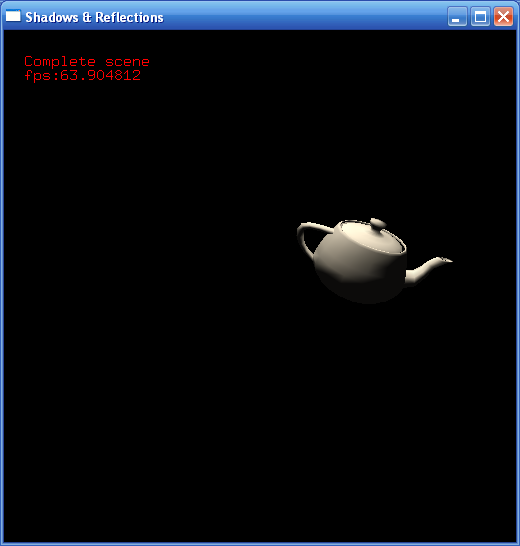
\includegraphics[width=8cm]{../exercise8/screenshots/1.png}
\caption{Det udleverede program}
\label{fig:8-1-1}
\end{figure}


\section{Part 2}

Vi skal nu implementere 2 funktioner:

\texttt{set_from_light_perspective(...)}\\
Funktionen laver en ``perspective projection'' som passer til objektet ud fra dens ``bounding sphere''.


\texttt{init_proj_shadow_texture(...)}\\
Initialiserer en texture som indeholder skyggen, opretter et texture name og ops�tter filters.

\section{Part 3}

\texttt{make_proj_shadow_texture(...) }

Thepotten renderes fra lyskilden og kopierer framebufferen til en textur.

\begin{figure}[hp]
\centering
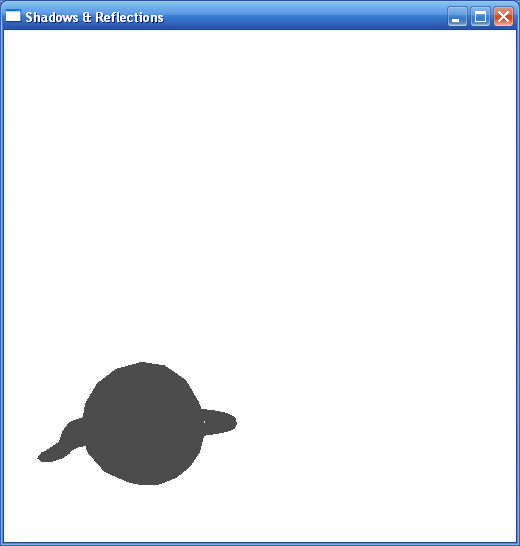
\includegraphics[width=8cm]{../exercise8/screenshots/3.png}
\caption{Skyggen}
\label{fig:8-3-1}
\end{figure}

\section{Part 4}

\texttt{draw_proj_shadow(...)}

Til sidst s�ttes det hele sammen. Farven i frame bufferen blandes med texturen.

Der er tilf�jet et clipping plane, s� skyggen ikke bliver vist hvis thepotten er under gulvet. Dette skal bruges i exercise 10.

\begin{figure}[hp]
\centering
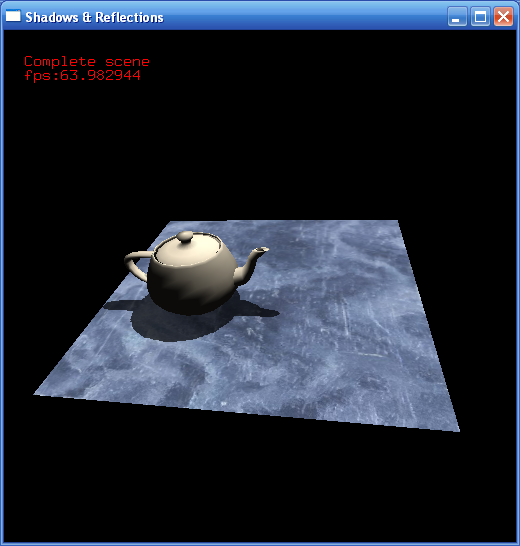
\includegraphics[width=8cm]{../exercise8/screenshots/4.png}
\caption{Det f�rdige program}
\label{fig:4-3-1}
\end{figure}